\documentclass[margin=0.5cm]{standalone}

\usepackage{tikz}
\usepackage{xcolor}

\usetikzlibrary{arrows.meta}


\begin{document}

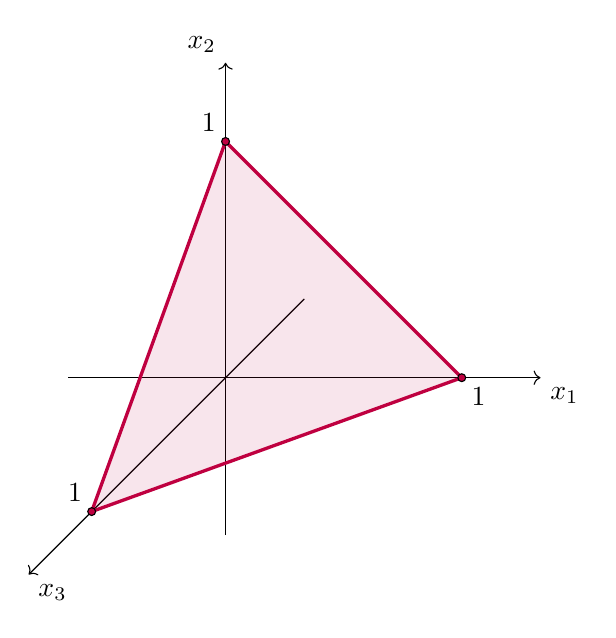
\begin{tikzpicture}
  \draw[->] (0,-2) -- (0,4);
  \draw[->] (-2,0) -- (4,0);
  \draw[->] (1.0,1.0) -- (-2.5,-2.5);
  \draw (0,4) node[anchor=south east] {$x_2$};
  \draw (4,0) node[anchor=north west] {$x_1$};
  \draw (-2.5,-2.5) node[anchor=north west] {$x_3$};

  \draw[purple, very thick, fill=purple, fill opacity=0.1] (0,3) -- (-1.7, -1.7) -- (3,0) -- (0,3);

  \draw[fill=purple] (0,3) circle[radius=0.05];
  \draw (0,3) node[anchor=south east] {$1$};
  \draw[fill=purple] (3,0) circle[radius=0.05];
  \draw (3,0) node[anchor=north west] {$1$};
  \draw[fill=purple] (-1.7,-1.7) circle[radius=0.05];
  \draw (-1.7,-1.7) node[anchor=south east] {$1$};
\end{tikzpicture} 

\end{document}
